\documentclass{article}
%\usepackage{geometry}
% \geometry{top = 1in, bottom = 1in, left = 1in, right = 1in}
\usepackage[top = 0.7in, bottom = 0.7in, left = 0.7in, right = 0.7in]{geometry}
\usepackage{amsmath,amssymb,amsthm,mathrsfs}
\usepackage{graphicx}
\usepackage{bm}
\usepackage{float}
\usepackage[font=footnotesize,labelfont=bf]{caption}
\usepackage{wrapfig}

\usepackage{hyperref} % For hyperlinking

\usepackage{fancyhdr}
\pagestyle{fancy}
\rhead{\footnotesize {May 2021; MESA version 15140} }
\chead{\footnotesize {Authors: Matteo Cantiello, Chris Mankovich \& Adam Jermyn} }
\lhead{\footnotesize {mesa/star/test\_suite/magnetic_braking} }
%----------------------------------------------------------------------------------------
%	MACROS
%----------------------------------------------------------------------------------------
% basic unit typesetteing
\newcommand{\unitspace}{\ensuremath{\,}}
\newcommand{\usp}{\unitspace}
\newcommand{\numberspace}{\ensuremath{\;}}
\newcommand{\nsp}{\numberspace}
\newcommand{\unitstyle}[1]{\ensuremath{\mathrm{#1}}}
\newcommand{\power}[2]{\ensuremath{{#1}^{#2}}}


% base units, mks
\newcommand{\meter}{\unitstyle{m}}
\newcommand{\second}{\unitstyle{s}}


% base units, cgs
\newcommand{\cm}{\centi\meter}
\newcommand{\gram}{\unitstyle{g}}

% solar and astronomical units
\newcommand{\Msun}{\ensuremath{M_\odot}}
\newcommand{\Lsun}{\ensuremath{L_{\odot}}}
\newcommand{\Rsun}{\ensuremath{R_{\odot}}}

% misc. units
\newcommand{\km}{\kilo\meter}   %kilometers
\newcommand{\Hz}{\unitstyle{Hz}}        %Hertz
\newcommand{\ksec}{\kilo\second} %kilosecond
\newcommand{\kms}{\ensuremath{\mathrm{km} \,\second^{-1}}}



\begin{document}
	
	\begin{center}
		\begin{Large}
		       \textbf{MAGNETIC BRAKING}\\
		\end{Large}
	\end{center}



This test case involves the calculation of the spin down caused by a large-scale magnetic field in a massive star model. 
The model has an initial mass of 15$\Msun$ and equatorial rotational velocity of 250 $\kms$ on the ZAMS. The angular momentum loss due to magnetic braking is calculated under simplifying assumptions (see below), resulting in a spin down of the model 
during its main sequence evolution.
The amplitude of the poloidal component of the magnetic field at the surface is 500 G (this is set by \texttt{x\_ctrl(1)} in \texttt{inlist\_braking}). With such magnetic field, the timescale for magnetic spindown is shorter than the main sequence lifetime of the model, 
which is expected to be slowly rotating when the core hydrogen fraction reaches 0.01 (stopping criterion). The test checks that the surface rotational velocity of the model is  $< 1 \kms$. 
More details about the physics and the implementation below.  

\section{Implementation of Magnetic Braking}




In the presence of mass-loss, angular momentum is removed by the material in the stellar wind, resulting in a spin-down effect.
This is quite important in massive stars, that are known to be rapidly rotating and have strong stellar winds.
Some of these stars have also been found to have large scale magnetic fields, with amplitudes between hundreds up 
to thousands of Gauss. 


In stars with surface magnetic fields, the presence of such field will interplay with the mass-loss.
In particular,  if the kinetic energy density in the wind is smaller than the magnetic energy density at the surface of the star, 
then the wind flow has to follow the magnetic field lines. This increases the co-rotation radius of the wind, so that the material will leave the stellar surface with a higher specific 
angular momentum (larger lever arm).  The co-rotation radius  roughly corresponds to the Alfv\'en radius $R_A$,
that in this problem corresponds to the location where the radial components of the field and the flow have equal energy density.



\begin{wrapfigure}{r}{0.33\textwidth}
  \begin{center}
    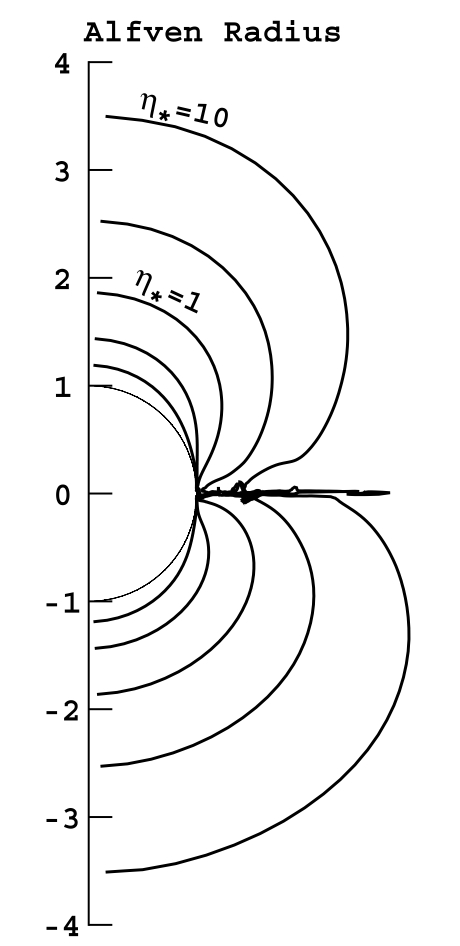
\includegraphics[width=0.31\textwidth]{uddoula.jpg}
  \end{center}
  \caption{Contours of the Alfv\'en radius as function of $\eta$ in the MHD models of ud-Doula \& Owocki \href{http://adsabs.harvard.edu/abs/2002ApJ...576..413U}{2002}}
\end{wrapfigure}




The angular momentum loss was first calculated, under simplified assumptions, by Weber \& Davis (\href{http://adsabs.harvard.edu/abs/1967ApJ...148..217W}{1967}) to 
study the angular momentum loss of the solar wind.
In their seminal work they found that the angular momentum lost by a magnetic rotator is:
\begin{equation}\label{jdot-eqn}
\dot J= \frac {2}{3} \dot M \Omega R_A^2 \, ,
\end{equation}
where $\Omega$ is the surface angular
velocity and  $\dot M$ is the mass-loss rate.
Detailed MHD calculations of this process have been performed, leading to more precise formulations (see e.g. ud-Doula \& Owocki \href{http://adsabs.harvard.edu/abs/2002ApJ...576..413U}{2002}, ud-Doula et al. (\href{http://adsabs.harvard.edu/abs/2008MNRAS.385...97U}{2008},\href{http://adsabs.harvard.edu/abs/2009MNRAS.392.1022U}{2009})).
However the scaling shown in Eq.~\ref{jdot-eqn} appears quite robust, and is therefore a good starting point 
to implement magnetic-braking in MESA.

It is useful to define the wind-confinement parameter $\eta$, the energy density ratio between radial magnetic field and flow
\begin{equation}\label{eta-eqn}
\eta(r) \equiv \frac{B_{r}^{2}/8\pi}{\rho v_{r}^{2}/2}
\, .
\end{equation}
This quantity can be rewritten at the stellar surface as $\eta_* = R_*^2\,B^2/\dot M\,v_\infty$,
where $v_\infty$ is the terminal velocity of the stellar wind. The line-driven winds of massive OB stars have 
terminal velocities that scale with the photospheric escape velocity ($v_\infty\simeq 1.92v_{\mathrm{esc}}$, see e.g. Lamers \& Cassinelli 2000), 
and are therefore of the order $\sim 1000-4000\,\kms$ or so. Using the wind confinement parameter,
it is possible to re-write Eq.~\ref{jdot-eqn} in a form that mostly only depends on values already calculated in MESA:
\begin{equation}\label{jdot-eqn2}
\dot J \approx \frac {2}{3} \dot M \Omega R_*^2 \eta_*\, ,
\end{equation}
 
The quantities  $\Omega$, $\dot M$, $R_*$ can be directly extracted from the \verb+Star_info+ data
structure. $B$ is a parameter and is set by  \verb+x_ctrl(1)+ in \texttt{inlist\_braking}  (we will  assume the magnetic field is constant during the evolution). $v_\infty$ can also be calculated self-consistently,
using the definition of the escape velocity: 
\begin{equation}
 v_\infty \simeq 1.92\,v_{\mathrm{esc}} = 1.92 \times 618 \,\bigg(\frac{\Rsun}{R_*}\,\frac{M_*}{\Msun}\bigg)^{1/2} \,\kms.
\label{vinf}
\end{equation}
Improvements to Eq.~\ref{jdot-eqn2} can be found in the series of
paper of ud-Doula et al. (\href{http://adsabs.harvard.edu/abs/2008MNRAS.385...97U}{2008},\href{http://adsabs.harvard.edu/abs/2009MNRAS.392.1022U}{2009}) 
or in Matt et al. \href{http://adsabs.harvard.edu/abs/2012ApJ...754L..26M}{2012}. But for this test we use this simpler approach.

The test case makes use of  the \texttt{other\_torque} routine and the \texttt{extra\_jdot} hook to extract the $\dot J$ associated with the magnetic braking from the stellar structure.
More details are provided in the comments of \texttt{src/run\_stars\_extras.f90}.

The evolution of the surface rotational velocity and total angular momentum of the model in the test case \texttt{magnetic\_braking} is shown in Fig.~\ref{vsurf}.
If you are keen,  run the main sequence evolution of this rotating $15\Msun$ 
including the magnetic torque for fields [B = 10 , 50, 100, 1000 G]. Plot the time evolution of total angular momentum 
and surface rotation velocity for the 4 cases. Try to compare with results in 
Meynet et al. \href{http://adsabs.harvard.edu/abs/2011A%26A...525L..11M}{2011}
 (for example their Fig.3). 
 
 
 

\begin{wrapfigure}{r}{1\textwidth}
  \begin{center}
    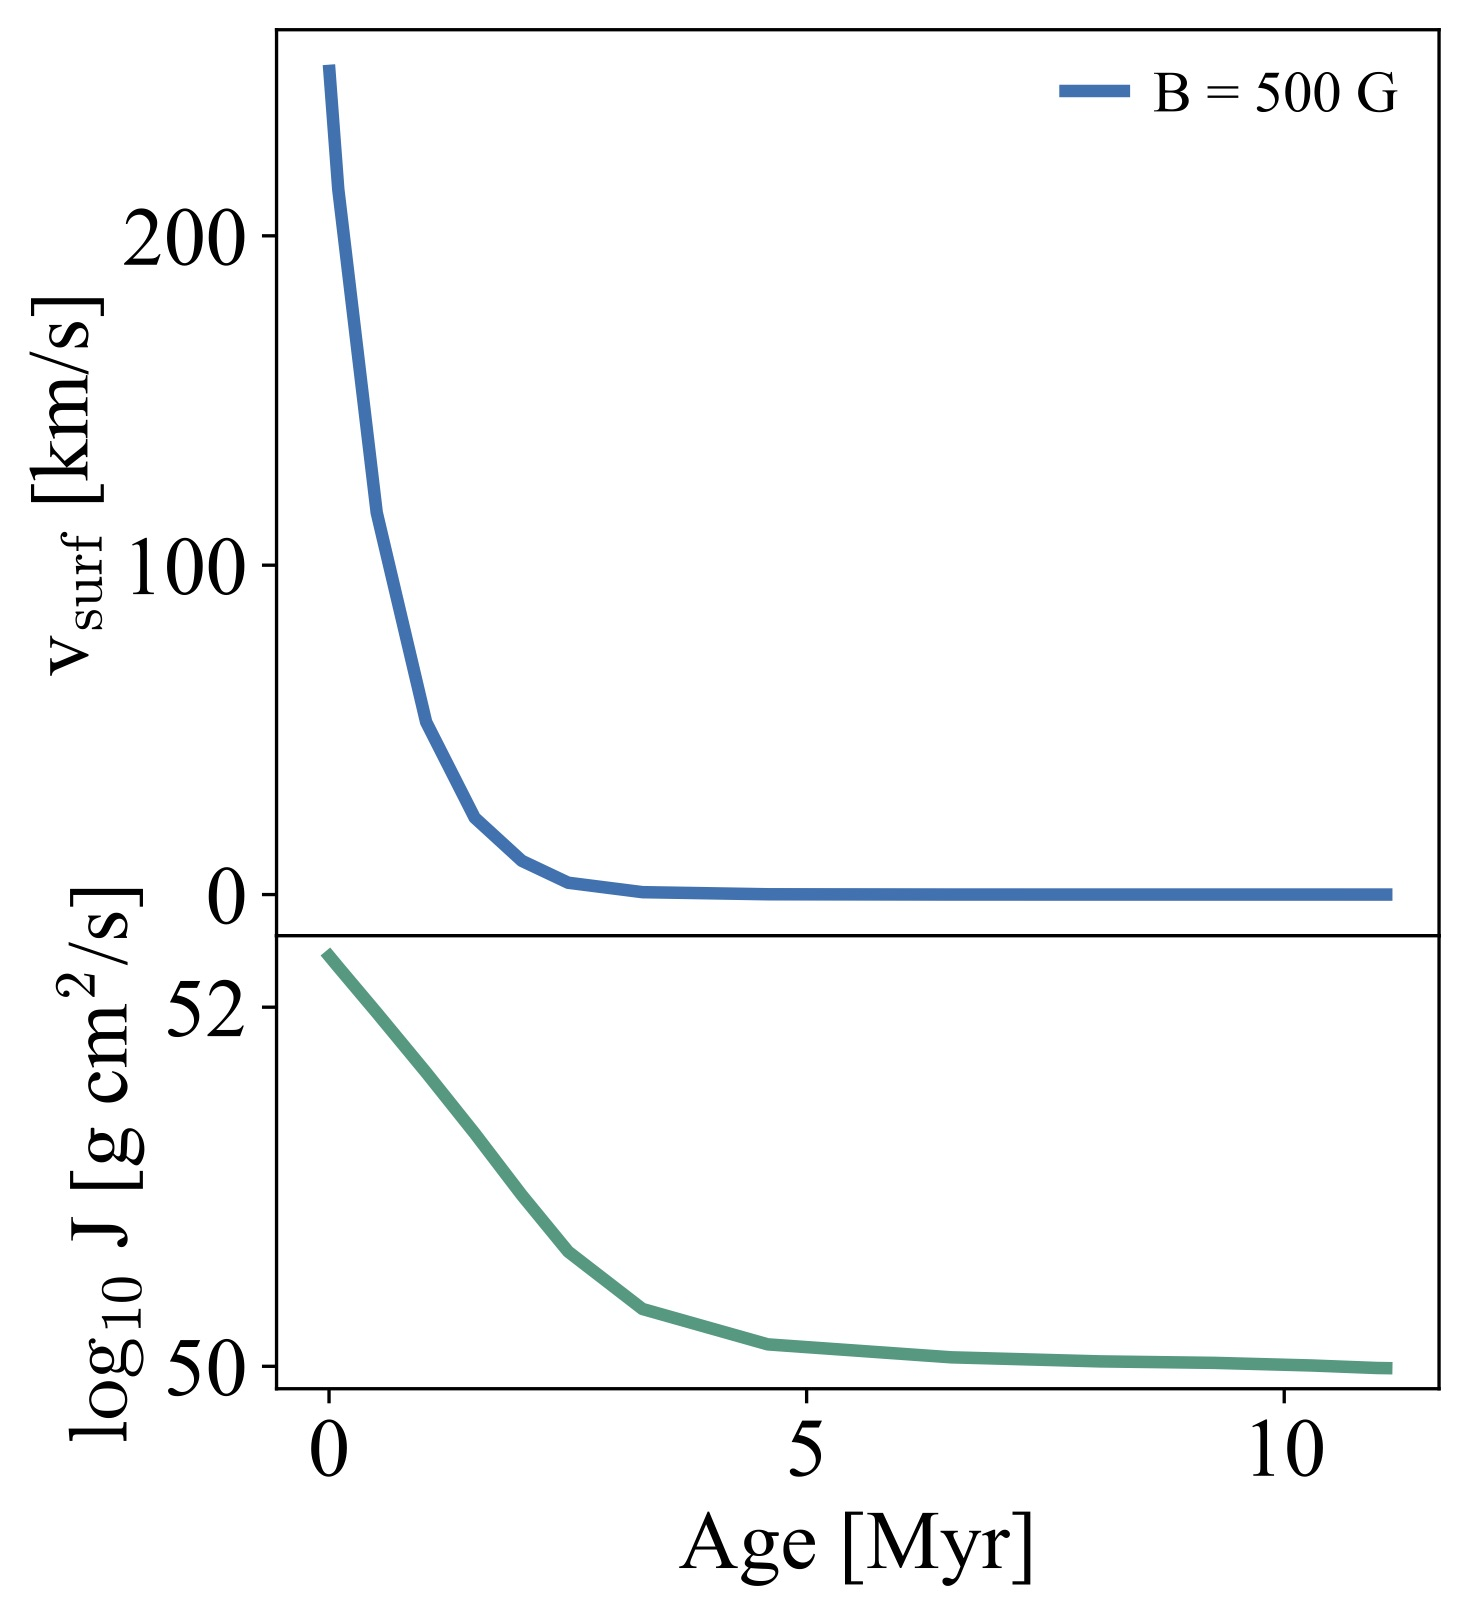
\includegraphics[width=0.9\textwidth]{vsurf.jpg}
  \end{center}
  \caption{Evolution of surface rotational velocity and total angular momentum for the model in the test case \texttt{magnetic\_braking}.}
  \label{vsurf}
\end{wrapfigure}

 
\end{document}